
\documentclass{standalone}

%Circular plate with distributed load
\usepackage{tikz}
\usepackage{pgfplots}
%\usepgfplotslibrary{patchplots}
%\pgfplotsset{compat=1.14}


\def\mystruct{\vphantom{hg}}

\pgfplotsset{
	legend image with text/.style={
		legend image code/.code={
		\node[anchor = center] at (0.3cm,0cm) {#1};
		}
	},width=15.5cm,height=7cm,compat=1.16,
}


\begin{document}



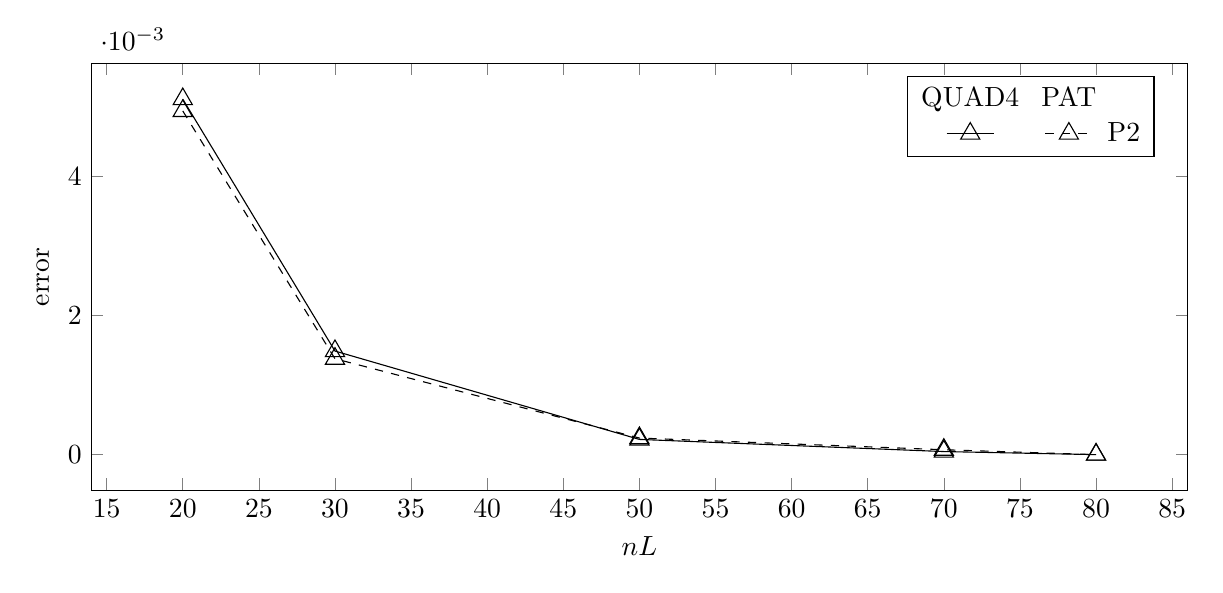
\begin{tikzpicture}
\begin{axis}[
%title={bla bla},
xlabel={$nL$},
ylabel={error},
name=boundary,
legend columns = 2,
legend style = {
		legend cell align = left,
		},
	legend pos = north east,
		%xmin=0,xmax=1.2,ymin=-15,ymax=1
]

\addlegendimage{legend image with text = QUAD4}
\addlegendentry{}

\addlegendimage{legend image with text = PAT}
\addlegendentry{}



%P2 _ REC
\addplot 
[solid,
mark=triangle,mark options = {scale = 2,solid},
]
coordinates {
(20,5.11113e-03)
(30,1.48934e-03)
(50,2.18933e-04)
(70,4.43600e-05)
(80,0.00000e+00)


};  \label{pgfplots:S_N_Tri}
\addlegendentry{}



%P2 _ TRI
\addplot 
[dashed,
mark=triangle,mark options = {scale = 2,solid},
]
coordinates {
(20,4.94101e-03)
(30,1.37871e-03)
(50,2.38535e-04)
(70,7.04771e-05)
(80,0.00000e+00)


};  \label{pgfplots:S_N_Tri}
\addlegendentry{P2}


%\addplot 
%[
%solid,mark options = {scale = 2,solid},
%]
%coordinates {(0,0)
%(32,0)
%};


\end{axis}

%\node [draw,fill=white,inner sep=0pt,above left = %0.5em ] at (boundary.south east) {\small
%\begin{tabular} {cc}
%fel & zdf \\
%\ref{pgfplots:C_SS_P_Tri} & %\ref{pgfplots:C_SS_P_Rec} \\
%\end{tabular}

%};


\end{tikzpicture}


\end{document}